% An appendix
%======================================================================
\chapter{X-ray Crystal Structures} \label{app.xrays}
\markright{X-Ray Crystal Structures}
%======================================================================

Multiple views of each x-ray crystal structure (including full unit cell) as discussed in \autoref{chap.newchem} are shown in \Cref{fig.xray21,fig.xray22,fig.xray23,fig.xray25,fig.xray28}. 

\begin{figure}[!ht]
 \centering
 \begin{subfigure}[b]{0.49\textwidth}
  \includegraphics[clip=true, width=\textwidth, height=50mm, keepaspectratio]{images/xray1a.eps}
 \end{subfigure}
 \begin{subfigure}[b]{0.49\textwidth}
  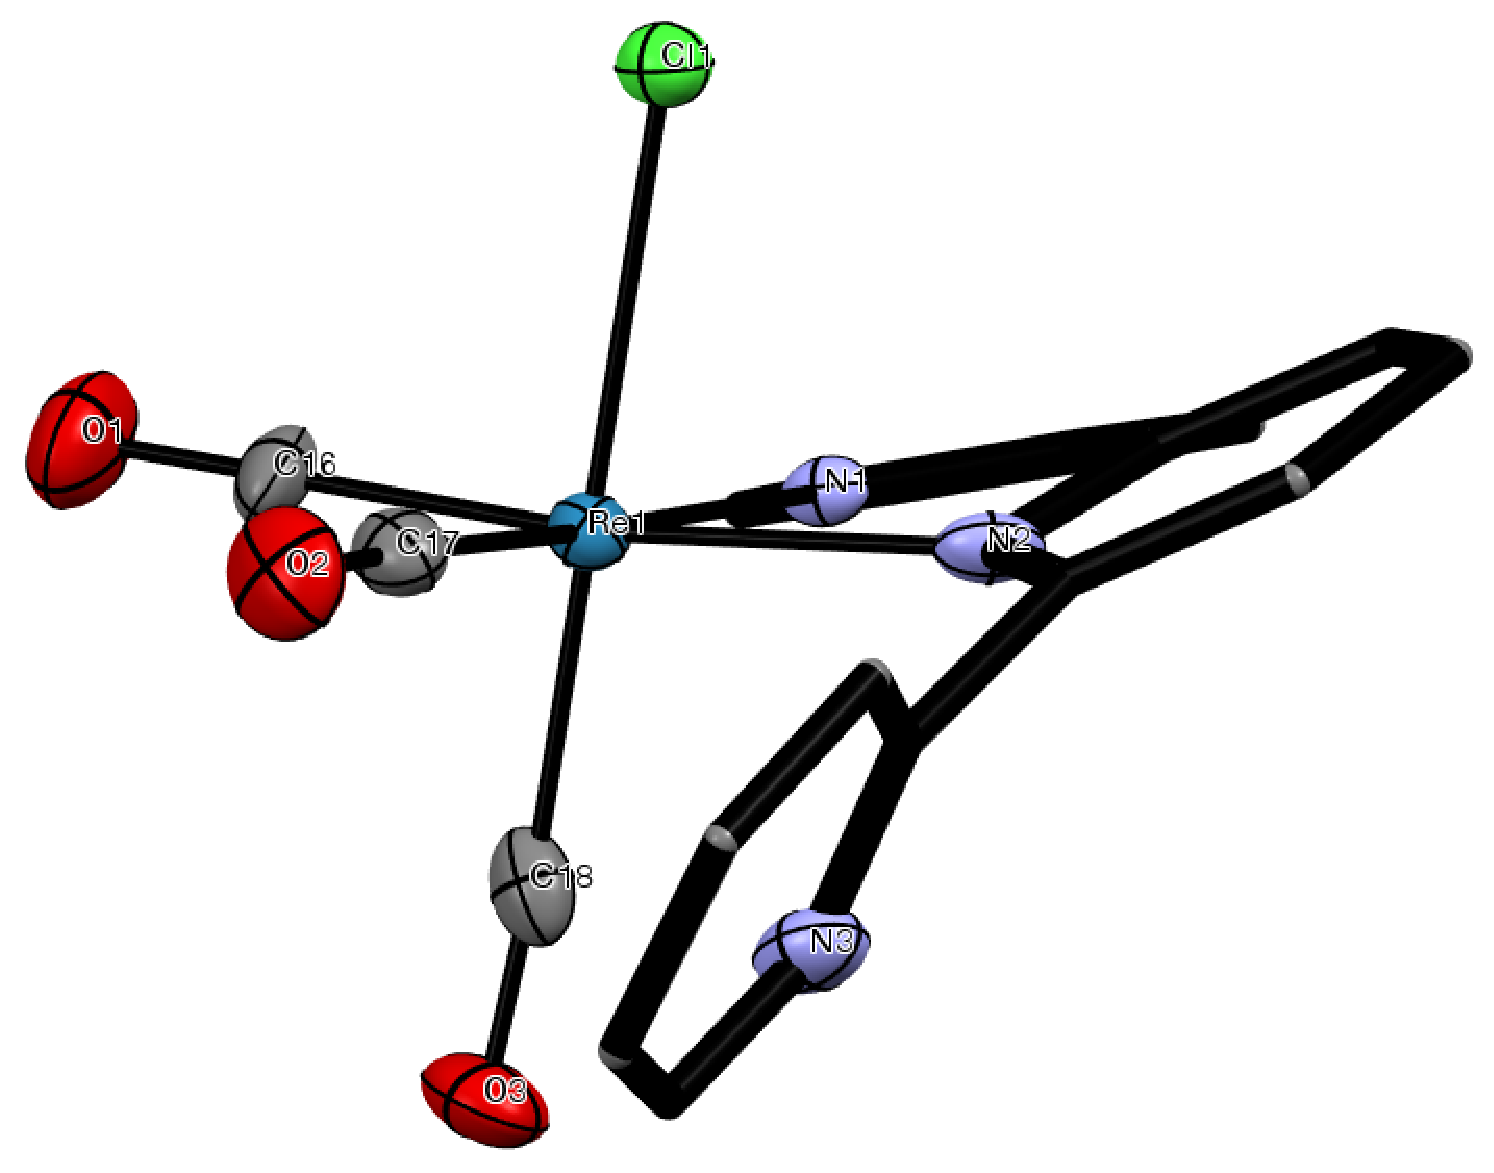
\includegraphics[clip=true, width=\textwidth, height=50mm, keepaspectratio]{images/xray1b.eps}
 \end{subfigure}
 \begin{subfigure}[b]{0.49\textwidth}
  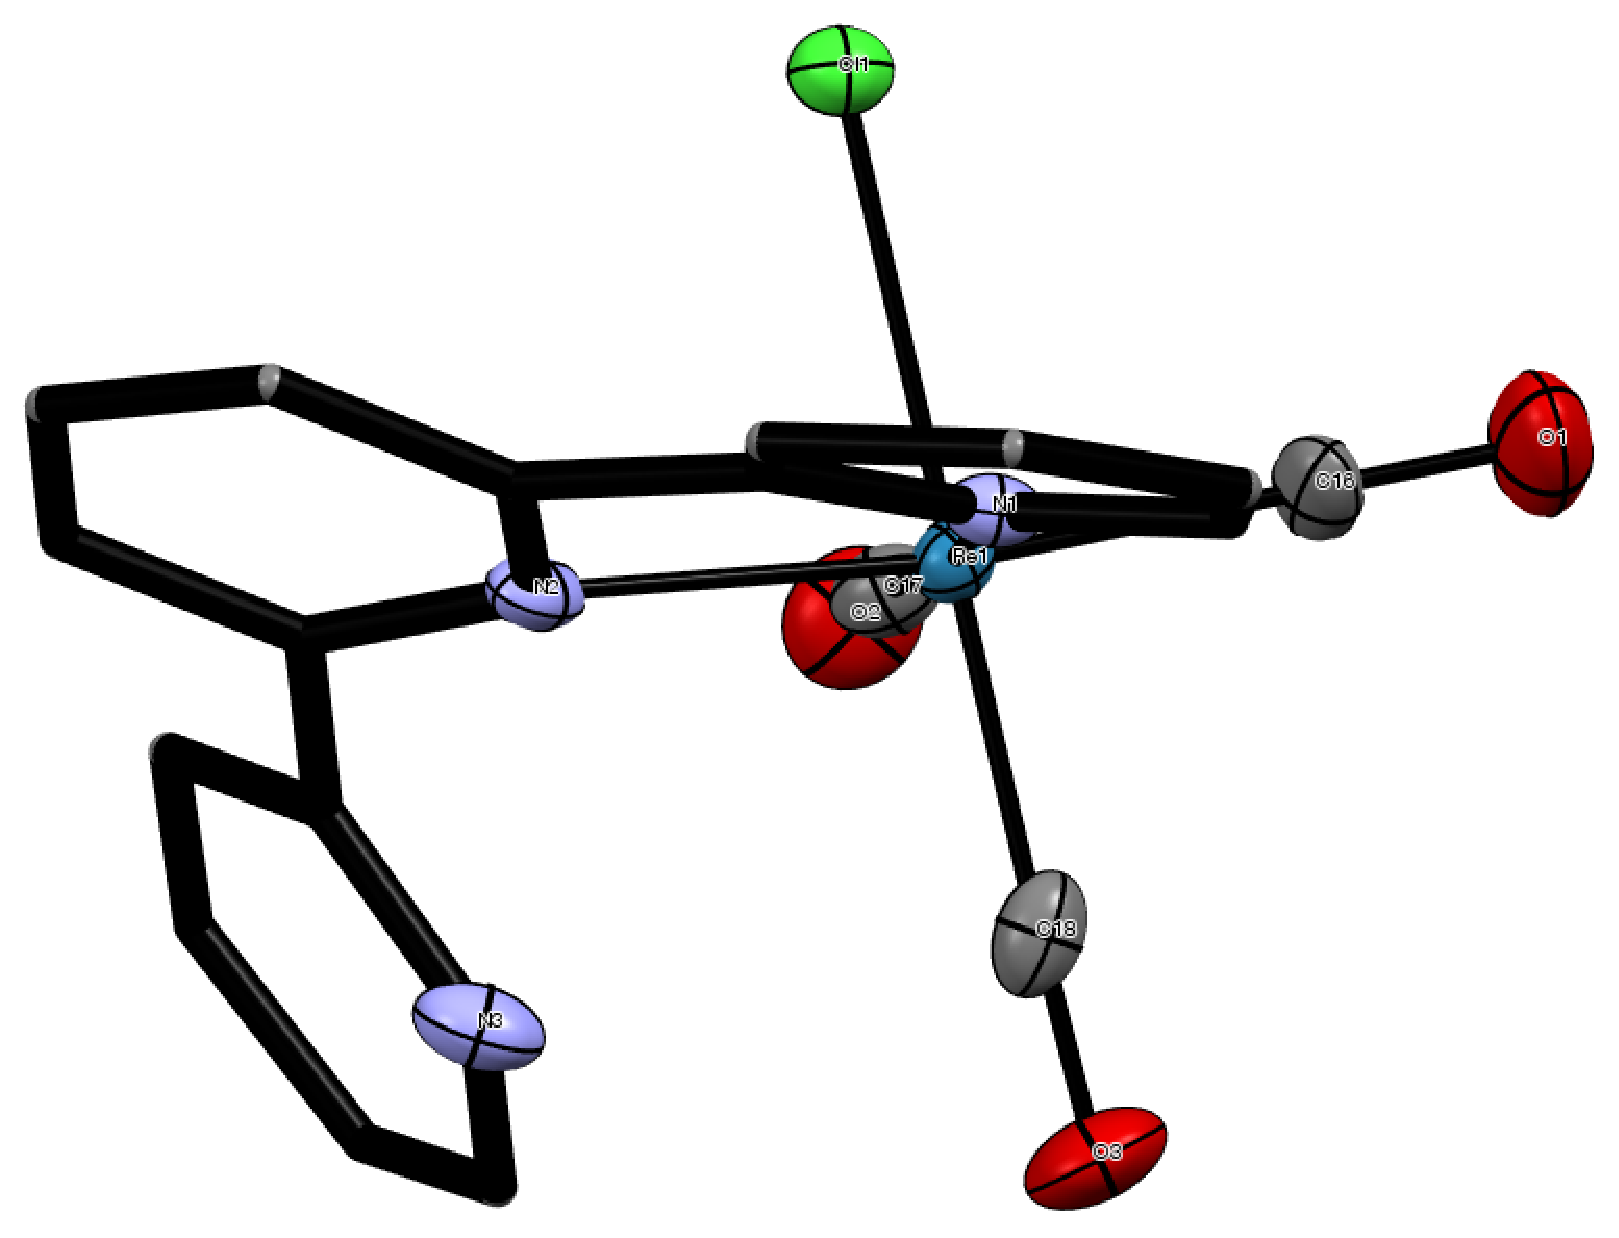
\includegraphics[clip=true, width=\textwidth, height=50mm, keepaspectratio]{images/xray1c.eps}
 \end{subfigure}
  \begin{subfigure}[b]{0.49\textwidth}
  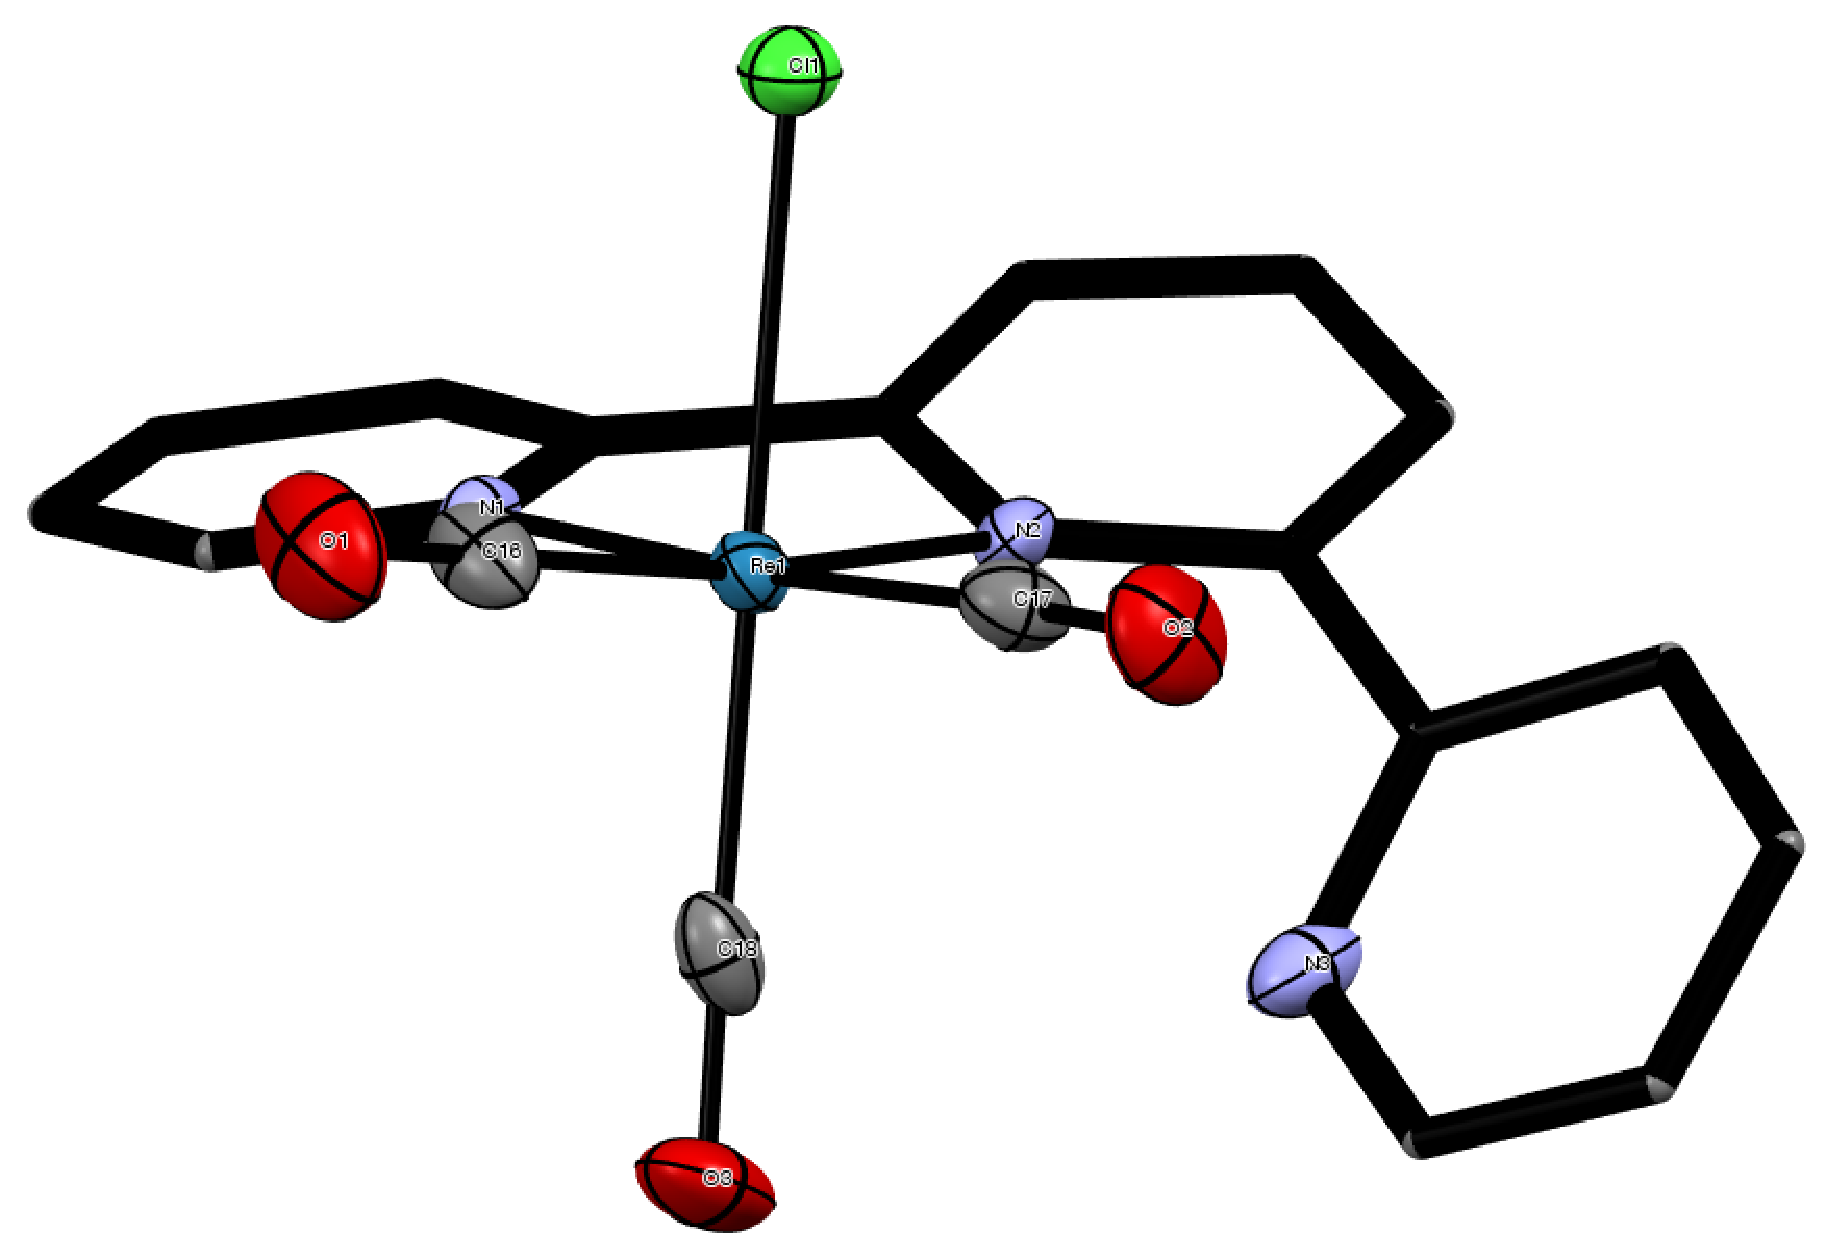
\includegraphics[clip=true, width=\textwidth, height=50mm, keepaspectratio]{images/xray1d.eps}
 \end{subfigure}
 \begin{subfigure}[b]{\textwidth}
  \centering
  \includegraphics[clip=true, width=\textwidth, height=75mm, keepaspectratio]{images/xray1uc.eps}
  \caption{Full unit cell representation of \textbf{2.1}.}
 \end{subfigure}
\caption[X-ray crystal structure of \textbf{2.1}.]{X-ray crystal structure of \textbf{2.1}. Co-crystallized chloroform, hydrogen atoms, and thermal ellipsoids of ligand carbon atoms are omitted for clarity.}
\label{fig.xray21}
\end{figure}

\begin{figure}[!ht]
 \centering
 \begin{subfigure}[b]{0.49\textwidth}
  \includegraphics[clip=true, width=\textwidth, height=50mm, keepaspectratio]{images/xray2a.eps}
 \end{subfigure}
 \begin{subfigure}[b]{0.49\textwidth}
  \includegraphics[clip=true, width=\textwidth, height=50mm, keepaspectratio]{images/xray2b.eps}
 \end{subfigure}
 \begin{subfigure}[b]{0.49\textwidth}
  \includegraphics[clip=true, width=\textwidth, height=50mm, keepaspectratio]{images/xray2c.eps}
 \end{subfigure}
 \begin{subfigure}[b]{\textwidth}
  \centering
  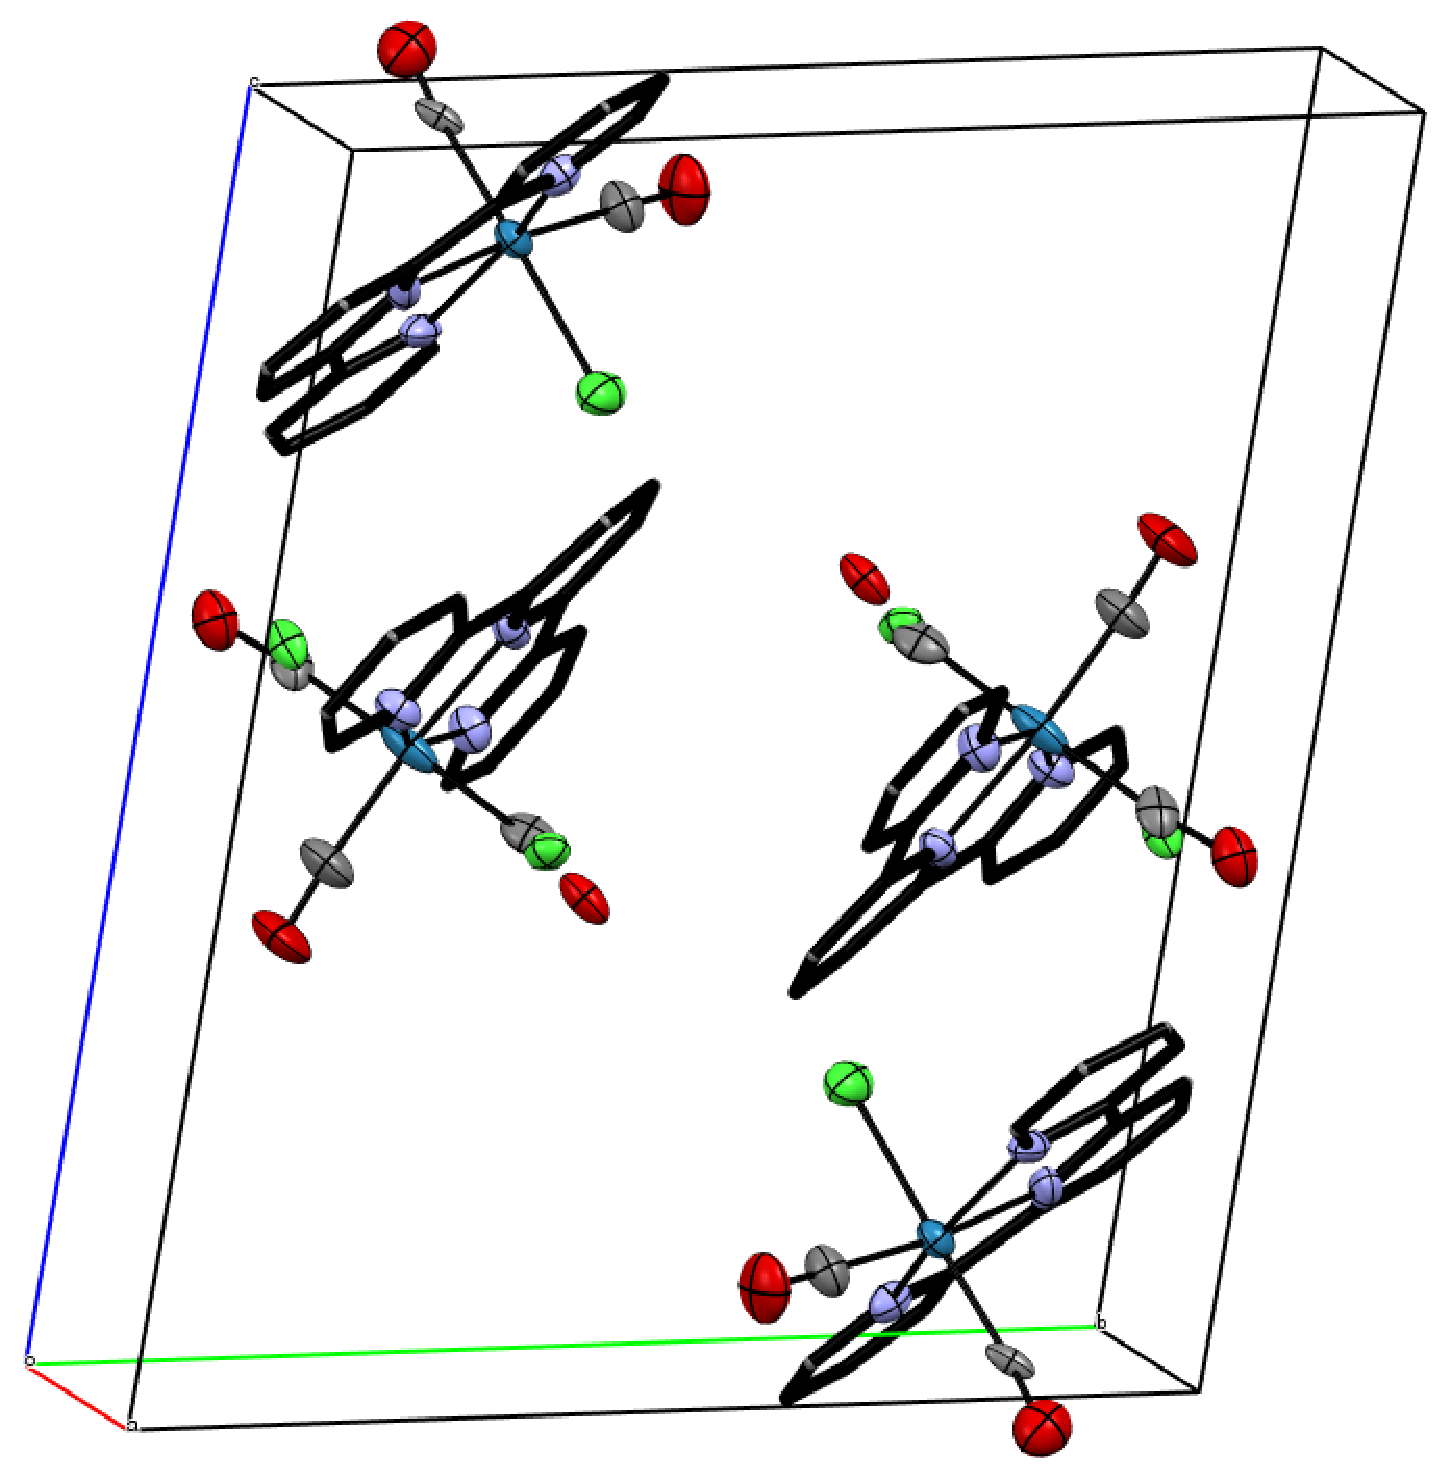
\includegraphics[clip=true, width=\textwidth, height=75mm, keepaspectratio]{images/xray2uc.eps}
  \caption{Full unit cell representation of \textbf{2.2}.}
 \end{subfigure}
\caption[X-ray crystal structure of \textbf{2.2}.]{X-ray crystal structure of \textbf{2.2}. Co-crystallized chloroform, hydrogen atoms, and thermal ellipsoids of ligand carbon atoms are omitted for clarity.}
\label{fig.xray22}
\end{figure}

\begin{figure}[!ht]
 \centering
 \begin{subfigure}[b]{0.49\textwidth}
  \includegraphics[clip=true, width=\textwidth, height=50mm, keepaspectratio]{images/xray3a.eps}
 \end{subfigure}
 \begin{subfigure}[b]{0.49\textwidth}
  \includegraphics[clip=true, width=\textwidth, height=50mm, keepaspectratio]{images/xray3b.eps}
 \end{subfigure}
 \begin{subfigure}[b]{0.49\textwidth}
  \includegraphics[clip=true, width=\textwidth, height=50mm, keepaspectratio]{images/xray3c.eps}
 \end{subfigure}
 \begin{subfigure}[b]{0.49\textwidth}
  \includegraphics[clip=true, width=\textwidth, height=50mm, keepaspectratio]{images/xray3d.eps}
 \end{subfigure}
 \begin{subfigure}[b]{\textwidth}
  \centering
  \includegraphics[clip=true, width=\textwidth, height=75mm, keepaspectratio]{images/xray3uc.eps}
  \caption{Full unit cell representation of \textbf{2.3}.}
 \end{subfigure}
\caption[X-ray crystal structure of \textbf{2.3}.]{X-ray crystal structure of \textbf{2.3}. Hydrogen atoms, and thermal ellipsoids of ligand carbon atoms are omitted for clarity.}
\label{fig.xray23}
\end{figure}

\begin{figure}[!ht]
 \centering
 \begin{subfigure}[b]{0.49\textwidth}
  \includegraphics[clip=true, width=\textwidth, height=50mm, keepaspectratio]{images/xray5a.eps}
 \end{subfigure}
 \begin{subfigure}[b]{0.49\textwidth}
  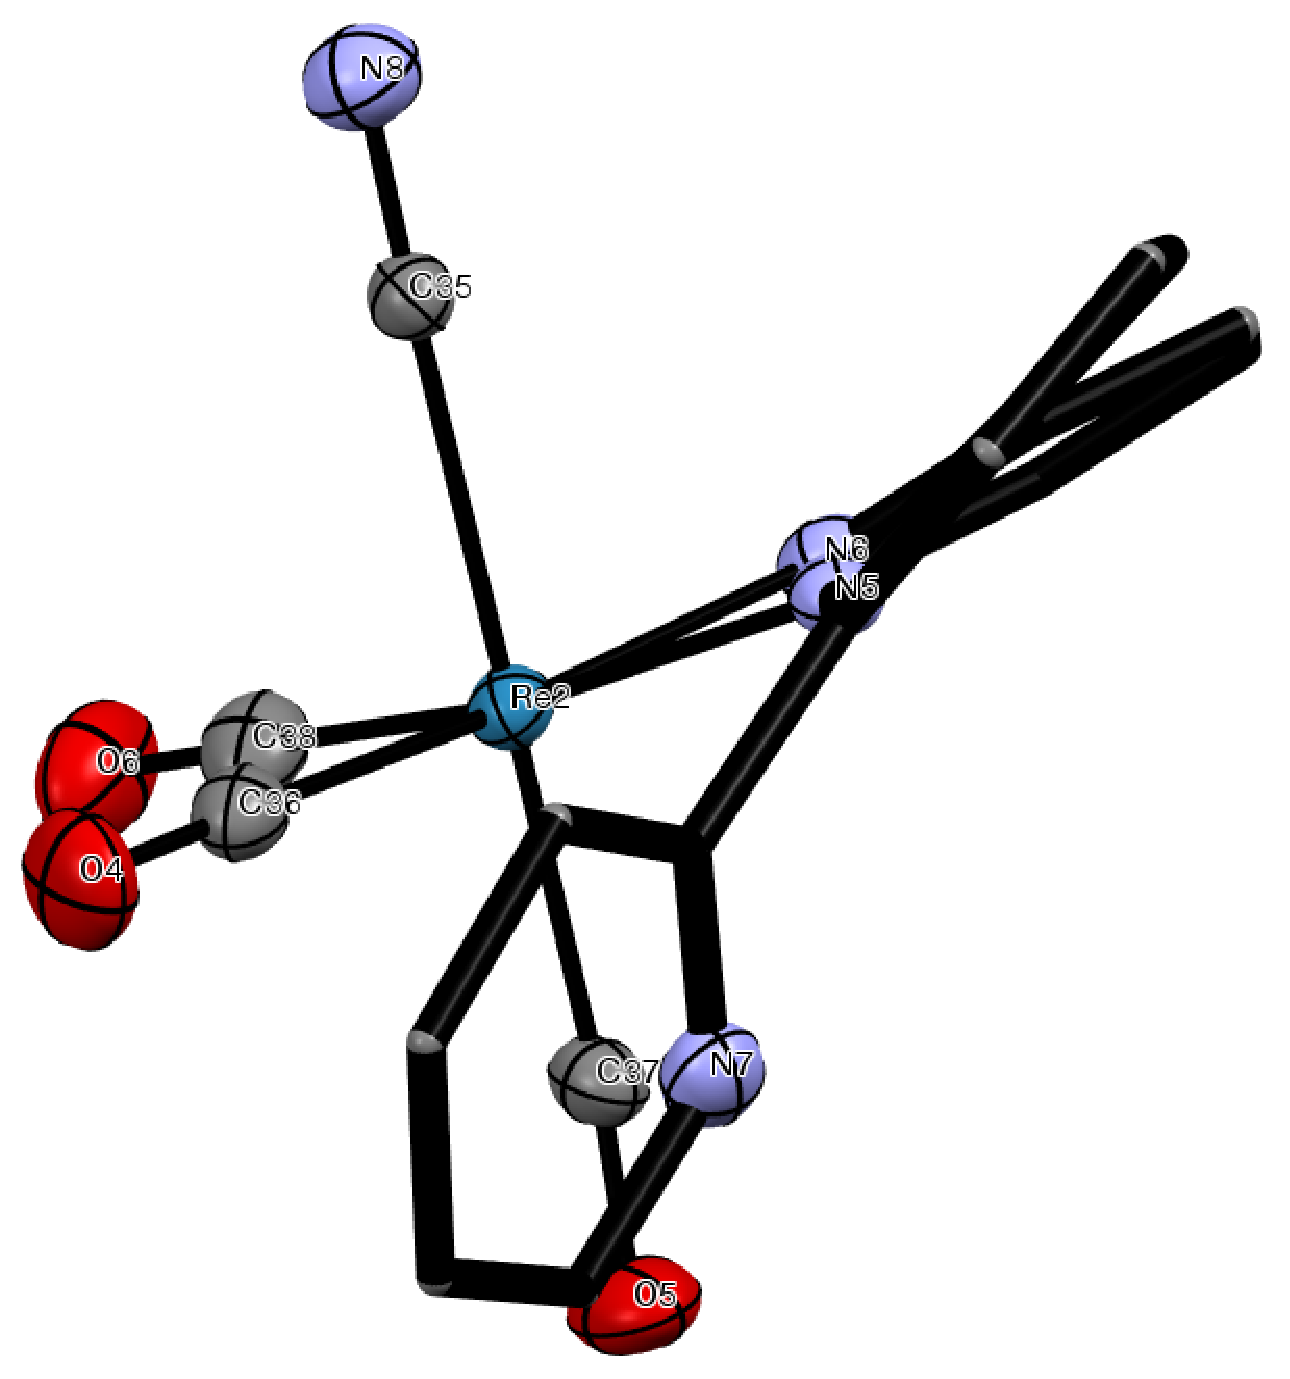
\includegraphics[clip=true, width=\textwidth, height=50mm, keepaspectratio]{images/xray5b.eps}
 \end{subfigure}
 \begin{subfigure}[b]{0.49\textwidth}
  \includegraphics[clip=true, width=\textwidth, height=50mm, keepaspectratio]{images/xray5c.eps}
 \end{subfigure}
 \begin{subfigure}[b]{0.49\textwidth}
  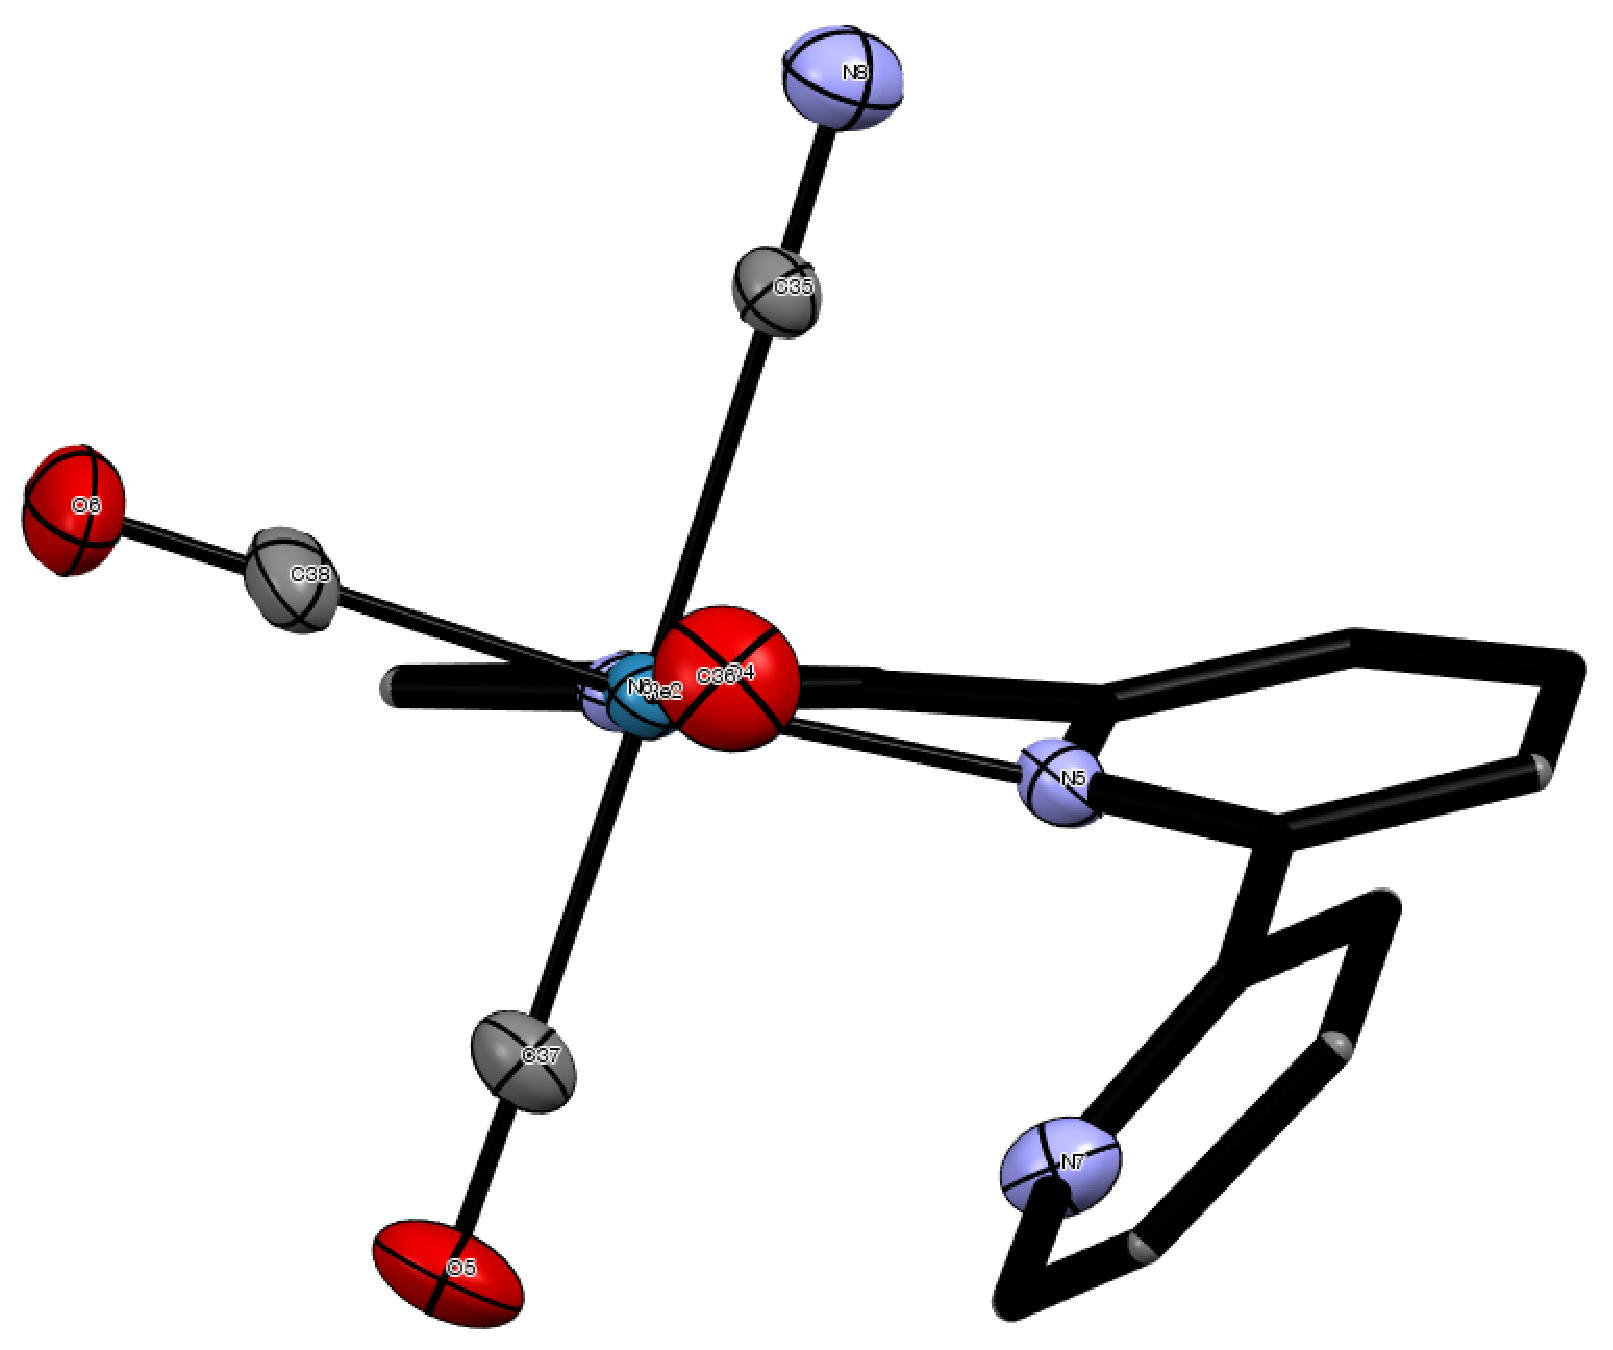
\includegraphics[clip=true, width=\textwidth, height=50mm, keepaspectratio]{images/xray5d.eps}
 \end{subfigure}
 \begin{subfigure}[b]{\textwidth}
  \centering
  \includegraphics[clip=true, width=\textwidth, height=75mm, keepaspectratio]{images/xray5uc.eps}
  \caption{Full unit cell representation of \textbf{2.5}.}
 \end{subfigure}
\caption[X-ray crystal structure of \textbf{2.5}.]{X-ray crystal structure of \textbf{2.5}. Hydrogen atoms, and thermal ellipsoids of ligand carbon atoms are omitted for clarity.}
\label{fig.xray25}
\end{figure}

\begin{figure}[!ht]
 \centering
 \begin{subfigure}[b]{0.49\textwidth}
  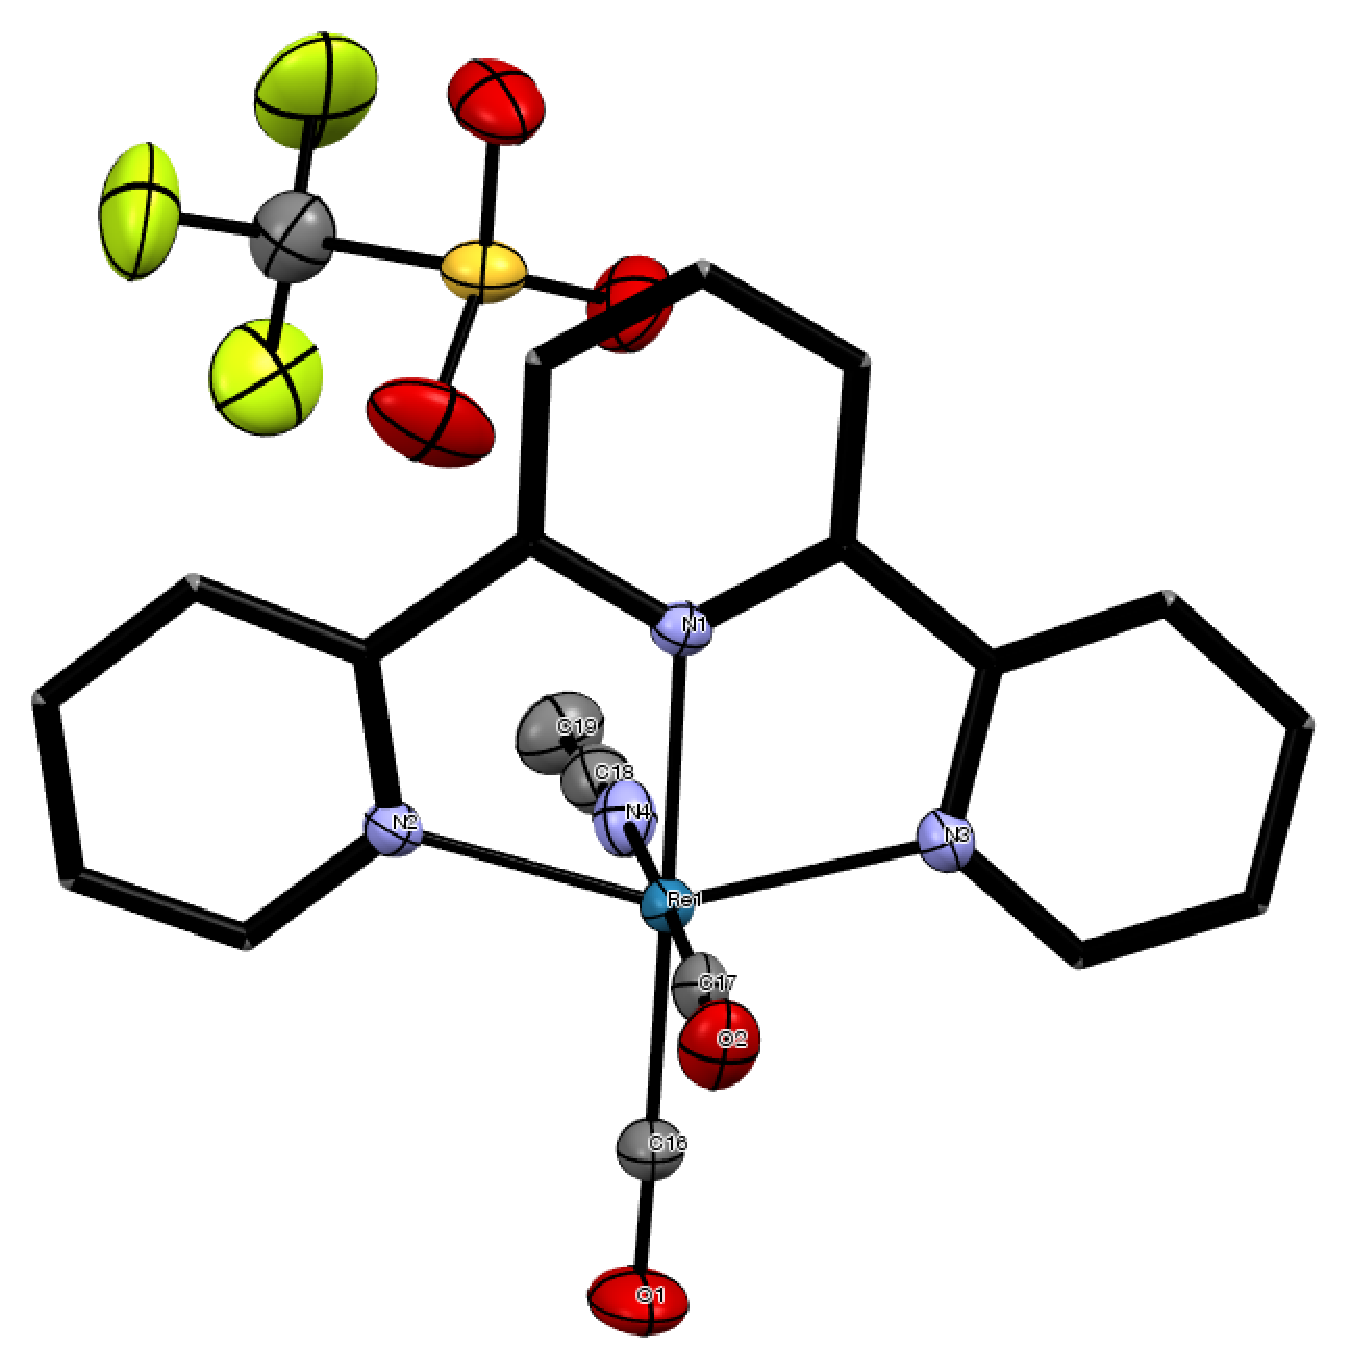
\includegraphics[clip=true, width=\textwidth, height=50mm, keepaspectratio]{images/xray8a.eps}
 \end{subfigure}
 \begin{subfigure}[b]{0.49\textwidth}
  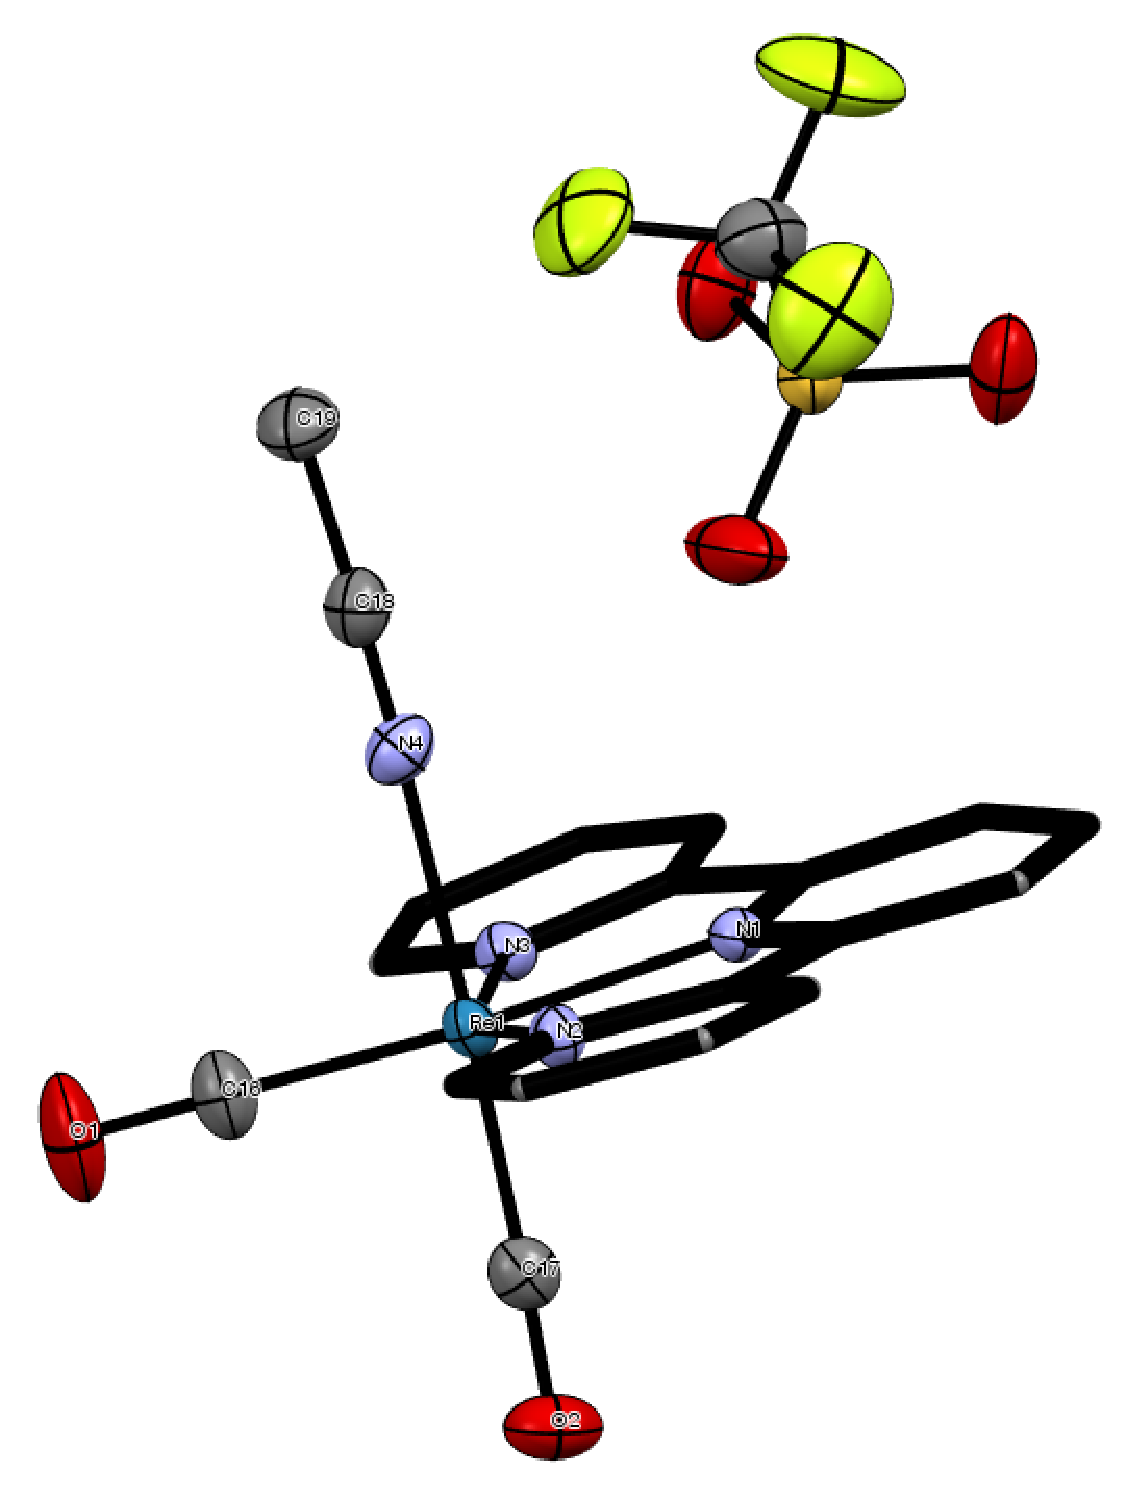
\includegraphics[clip=true, width=\textwidth, height=50mm, keepaspectratio]{images/xray8b.eps}
 \end{subfigure}
 \begin{subfigure}[b]{0.49\textwidth}
  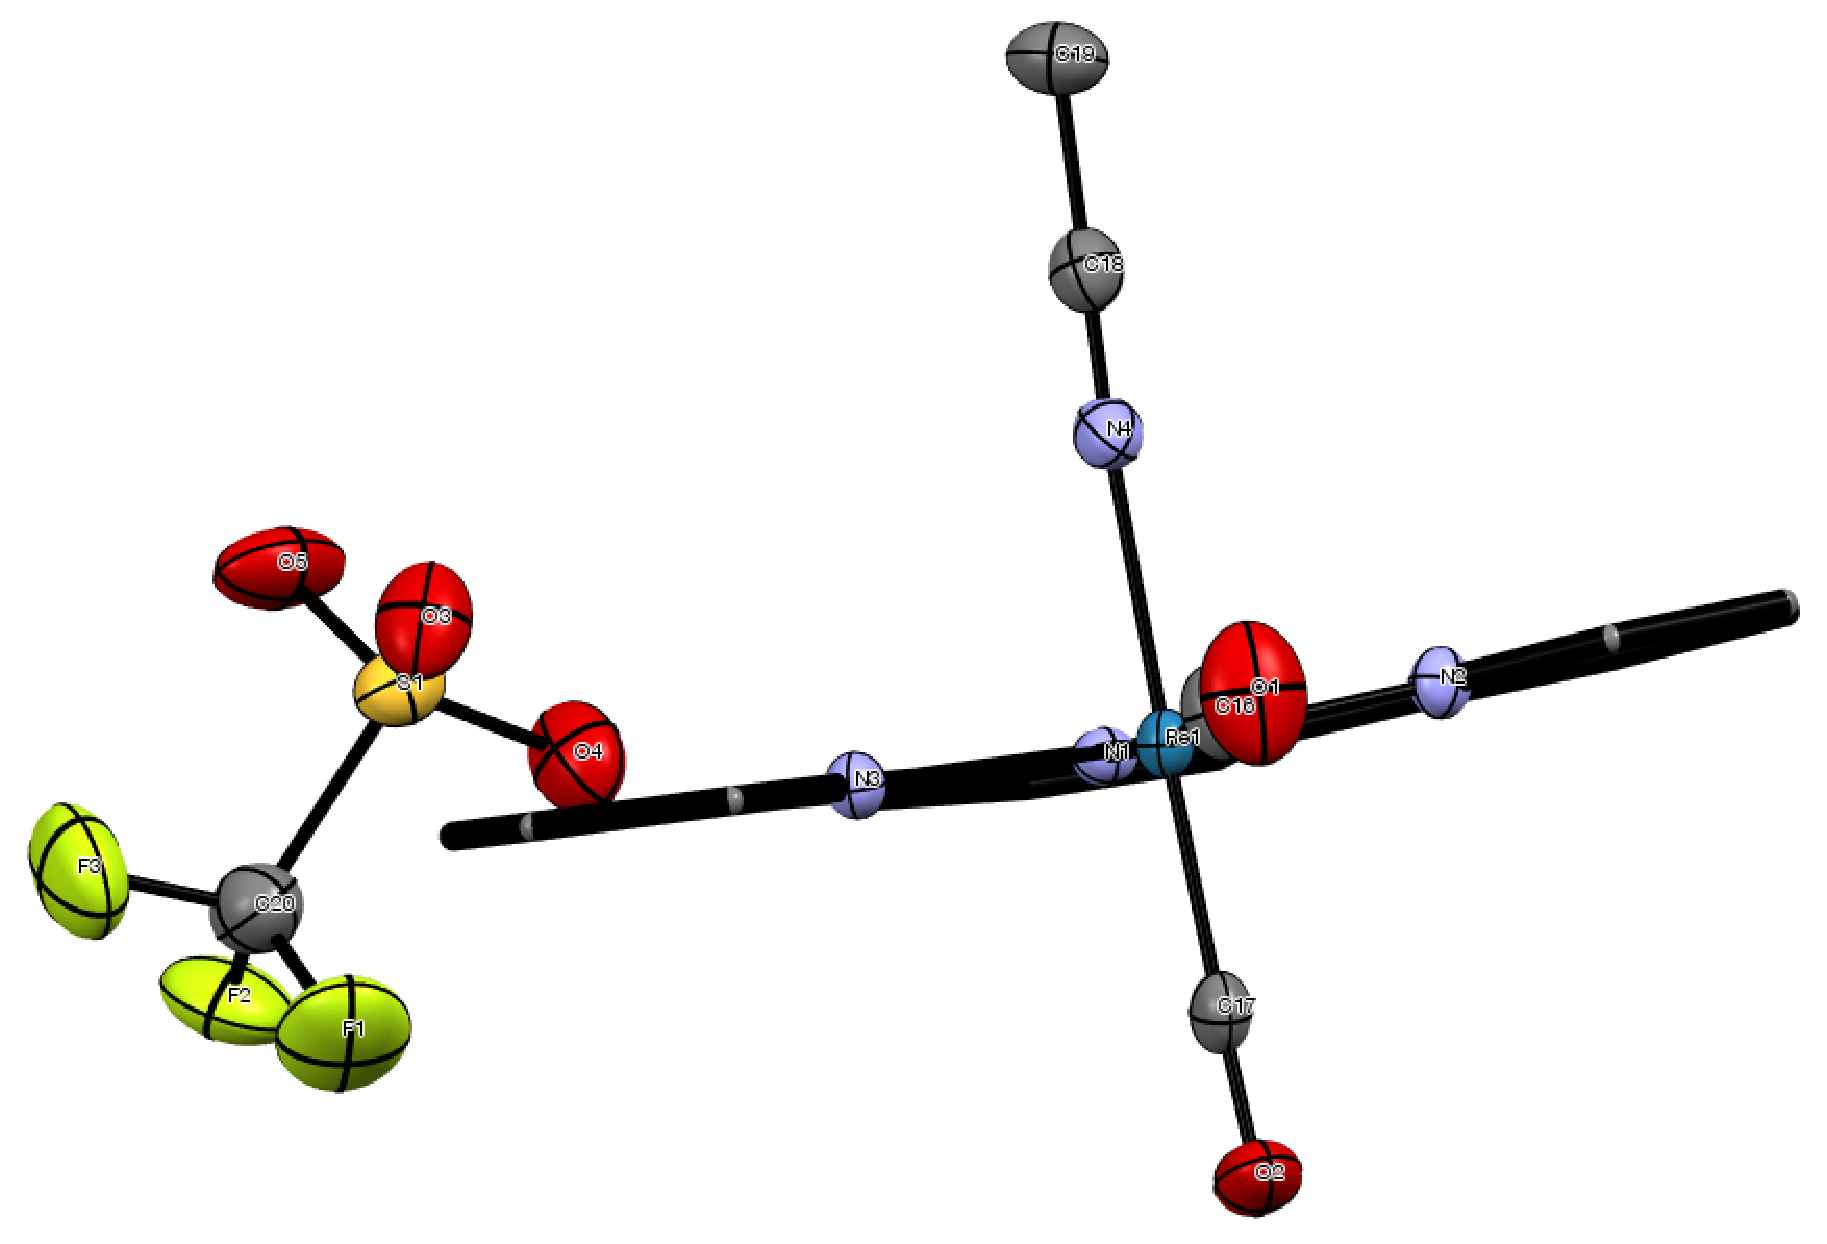
\includegraphics[clip=true, width=\textwidth, height=50mm, keepaspectratio]{images/xray8c.eps}
 \end{subfigure}
 \begin{subfigure}[b]{0.49\textwidth}
  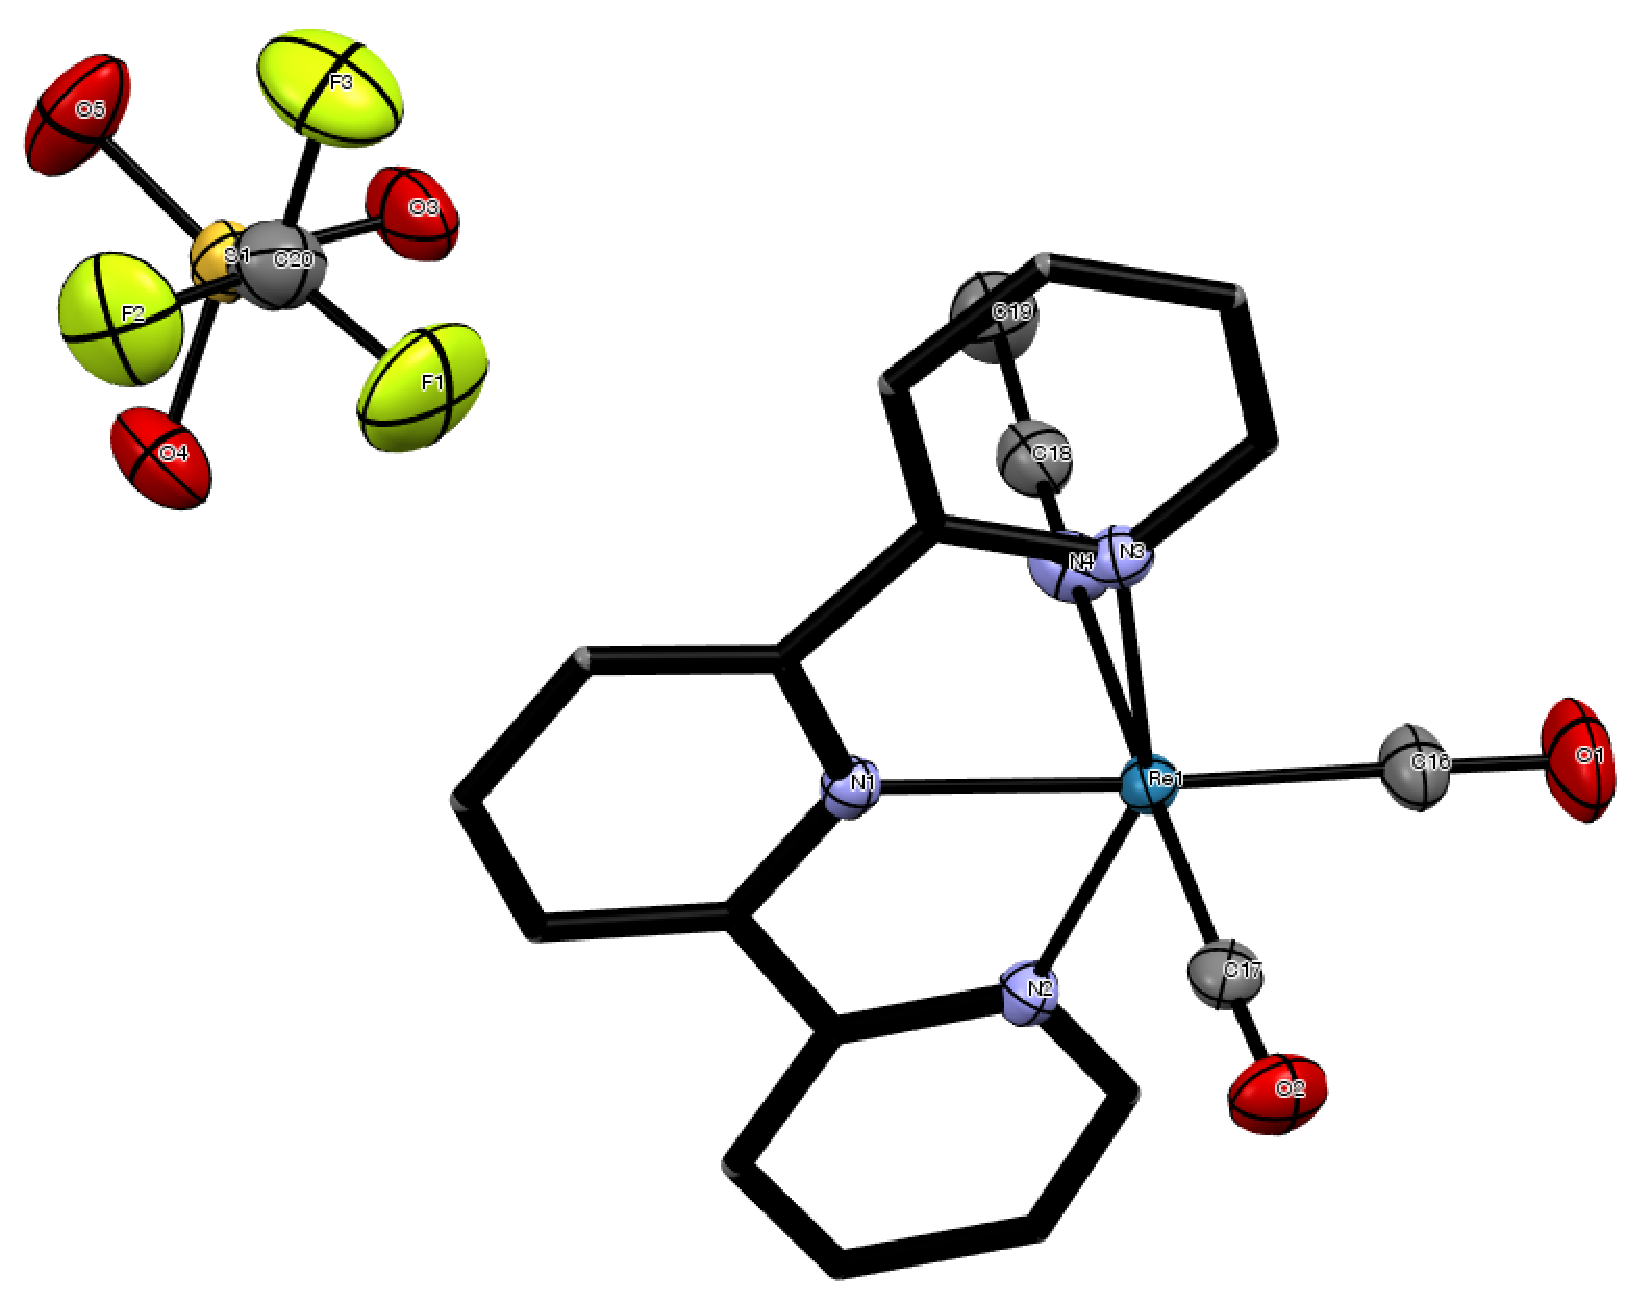
\includegraphics[clip=true, width=\textwidth, height=50mm, keepaspectratio]{images/xray8d.eps}
 \end{subfigure}
 \begin{subfigure}[b]{\textwidth}
  \centering
  \includegraphics[clip=true, width=\textwidth, height=75mm, keepaspectratio]{images/xray8uc.eps}
  \caption{Full unit cell representation of \textbf{2.8}.}
 \end{subfigure}
\caption[X-ray crystal structure of \textbf{2.8}.]{X-ray crystal structure of \textbf{2.8}. Hydrogen atoms, and thermal ellipsoids of ligand carbon atoms are omitted for clarity.}
\label{fig.xray28}
\end{figure}